\documentclass[pdftex,12pt,letter]{article}
\usepackage{fancyhdr}
\usepackage{enumerate}
\usepackage{tabularx}
\usepackage{graphicx}
\usepackage{array}
\usepackage[justification=justified,singlelinecheck=false]{caption}
\usepackage{placeins}
\pagestyle{fancy}
\makeatletter
  \renewcommand\@seccntformat[1]{\csname the#1\endcsname.\quad}
\makeatother

\newcolumntype {Y}{ >{\raggedright \arraybackslash }X}
\newcommand{\HRule}{\rule{\linewidth}{0.5mm}}
\captionsetup{labelformat=empty}

\begin{document}

\begin{titlepage}
\begin{flushright}
\HRule \\[0.4cm]
{ \bfseries
{\huge Inspection Report\\[1cm]}
{\large Reviewed by\\Jason Kuster, Stuart Long, and William Ordivay\\
\normalsize Moderated by Adrian Bubie}\\[1cm]
\normalsize Conducted at 11:33 pm on October 25th 2012}\\[1cm]
KOALAA Development\\[1cm]
October 1, 2012
\end{flushright}
\end{titlepage}
\begin{flushleft}
\section{Introduction}
\subsection{Purpose}
This Inspection by Stuart Long, Jason Kuster, and William Ordiway lists changes that KOALAA would like to see in CWRUtility Requirements Specification Document 1.0
\section{Inspection Action Log}

{\small 
\begin{tabular}{|r|c|l|p{6cm}|}
    \hline
Location & Severity & Type & Description \\
  \hline
  Title Page & Min & Typo & Ordiway is spelt wrong \\
    \hline
  Section 1.1 & Min & Typo & Solo is misspelled \\
   & Min & Typo & Correction is misspelled \\
   & Min & Redundancy  &  delete "documented here are high priority" \\
  \hline
  Section 2.1 & Med & Rephrasing & Replace "emcompassing 'all'" with 'most'\\
  \hline
  Section 2.2 & Min & Rephrasing & change 'app' to 'applications'\\
    & Min & Typo & delete duplicate 'is'\\
    & Min & Rephrasing & Change "installed users" to "people who have installed the application"\\
    & Min & Rephrasing & Change "the background" to "pulls data from each service"\\
\hline
	Section 2.3 & Min & Rephrasing & change 'shall' to 'will'\\
	\hline
	Section 2.5 & High & Change to Feature & Remove the tutorial feature\\
	\hline
Section 3.1.1 & Min & Typo & uncapitalize 'user'\\
 & Min & upcapitalize 'serivice'\\
\hline
Section 3.2.1 & Min & Tense & change 'should be' to 'will be'\\
& Min & Grammar & "This" should have a noun after it\\
& Min & Grammar & Change 'but' to 'but also'\\
& Min & Grammar & delete 'as well'\\
& Min & Aesthetics & insert a line break at the end of the sentence\\
& High & Change to Feature & Removal of mapping navigation\\
& Mid & Aesthetics & FIXME \\ 
& Med & Formatting & list a priority for this section\\
\hline
Section 3.2.2 & Mid & Formatting & delete line breaks, change formatting so it is consistent with the rest of the document\\
 & High & Change to Feature & Delete Map.Navigate\\
\hline


\end{tabular}
}

\newpage

\begin{tabular}{|r|c|l|p{6cm}|}
\hline
Section 3.3.1 & High & Redefined & Change the nextbus section to reflect that CRWRUtility will be implimenting nextbus data into its UI and not simply embedding nextbus into the application\\
& Med & Formatting & list a priority for this section\\
& Min & Rephrasing & change 'open application' to 'open feature'\\
& High & Change to Feature & add 'select stop', 'route' and 'bus direction'  to functional requirements\\
\hline
Section 3.4.1 & Min & Rephrasing & change 'location' to 'locations'\\
\hline
Section 3.4.3 & Min & Grammar & 'phone numbers' should be plural\\
& Min & Rephrase & reword the Director.Call \\
\hline
Section 3.5.1 & Min & Rephrase & delete the 'of' in "will layout of the menus"\\
& Min & Typo & change to "dinning hall"\\
& Min & Rephrasing & change to "user selects a dinning hall to view"\\
& Med & Formatting & deleted \textit{The Case Daily}\\
& High & Change to Feature & change the priority of the 5YearCal to "lowest"\\
\hline

\end{tabular}


\end{flushleft}

\lfoot{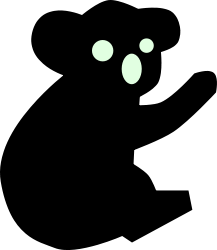
\includegraphics[height=1cm]{DarkKoala.png}}
\end{document}